\documentclass[10pt,letterpaper]{article}
\usepackage{geometry}
\geometry{margin=1in}
\usepackage{graphicx}
\usepackage{float}

\setlength{\parindent}{0pt}
\setlength{\parskip}{0.5em}

%make lists tighter
\usepackage{enumitem}
\setlist{nolistsep}

%reduce spacing before and after section
\usepackage{titlesec}
\titlespacing\section{0pt}{6pt}{0pt}

\title{Lab 1 - PECARN TBI Data, STAT 215A, Fall 2026}


\begin{document}
\maketitle

\section{Introduction}\label{introduction}

Traumatic brain injury (TBI) is one of the main causes of death and adverse outcomes in children, and around 50\%
of children presenting in emergency departments in the US are given CT scans to diagnose TBI \cite{Kuppermann2009}. This is despite the fact that
only 10\% of CT scans in children with minor head trauma actually show evidence of TBI and only a small proportion of these children go on to actually require surgery \cite{Kuppermann2009}.
On the other hand, CT scans expose children to ionizing radiation, which is especially detrimental to younger children (although risk decreases as age goes up).
Thus, there is great value in studying the TBI data to ultimately develop a clinical decision rule that can be used to identify pediatric patients that likely do not have
TBI and thus do not need to be exposed to the harmful effects of CT scans.


In our exploratory data analysis, we seek to understand what covariates are most predictive of TBI in children (to identify who actually needs a CT scan) and we
also investigate if there are any subgroups of children that are more likely than other groups to receive a CT scan.
The TBI data is quite messy and has many missing values that are not properly coded, which makes the analysis challenging. The rest of the report will be
is structured as follows: 1) describing the data, 2) cleaning and exploring the data it in an iterative process, 3) and then demonstrating the predictability
and stability of our initial findings and modeling.


\section{Data}\label{data}

This is a patient-level dataset of children (younger than 18 years old) who presented to the emergency department within 24 hours of trauma to the head, with 43,399 observations and 125 variables in the raw dataset.
The data was collected from 25 different emergency departments in PECARN, a federally funded network for conducting pediatric emergency medicine research \cite{pecarn}. The dataset
contains clinical and demographic information, patient history, and symptoms; this information was collected by ED doctors and site investigators on a standardized data form. According to the data documentation,
certain pediatric patients were excluded from the dataset: specifically, those with injury mechanisms that were classified as ``trivial'', those displaying no signs of head trauma besides abrasions/lacerations, and those with other
conditions (e.g., brain tumors, bleeding disorders, neurological conditions, etc.) that would not constitute ``good'' data to learn a clinical decision rules from for the typical pediatric patient \cite{Kuppermann2009}.
The dataset also contains the relevant CT results for the 15,899 patients for whom a CT scan was performed as well as the final clinical outcome, which was defined as ``clinically important traumatic brain injury'' (ciTBI).
See \cite{Kuppermann2009} for a detailed definition of ciTBI.

This dataset is clearly related to the problem of interest: if we seek to develop (or at least validate a clinical decision rule) for identifying head-injured children with low risk of ciTBI with the hopes of reducing unnecessary CT scans, it will be important to identify
which covariates are indicative of low risk (or on the other hand, high risk) of ciTBI and if there are any covariates that are predictive of receiving a CT scan when it is not necessary. Our raw dataset contains exactly this information.

\subsection{Data Collection}\label{data-collection}

The data was collected by ED doctors and ``site investigators'', who used a standardized data form to collect information about the patient's history, injury mechanism, and symptoms \cite{Kuppermann2009}.
This process was completed before knowing imaging results if imaging was performed. To ensure data quality and accuracy, around 4\% of patients were evaluated by another physician within the first hour of their
initial evaluation \cite{Kuppermann2009}. The data was collected from 25 emergency departments, and the entire dataset spans from June 2004 through September 2006, although the dataset itself is not indexed by time \cite{Kuppermann2009}. Notably, most of the
hospitals in the study were pediatric hospitals, which have a CT rate that is lower than that of non-pediatric hospitals.

Naturally, the measurements of each variable, even for the same observation, may vary due to different ED physicians' clinical judgment. Particularly, two of the variables, dizziness and scalp hematoma, are two extreme examples that had especially poor inter-observer agreement.
Additionally, the researchers in this study were not able to obtain a CT scan for every patient, which would have been a more definitive ``ground truth'' value. Instead, if the patient was discharged
from the ED, the researchers followed up with the patient's guardians or other medical records to determine the patient's ciTBI classification. If the patient was admitted to the inpatient hospital, the researchers similarly reviewed medical records
to assess if ciTBI was present.


\subsection{Data Cleaning}\label{data-cleaning}

We start by filtering the dataset to only include patients with a GCS score of 14 or 15. This is the ``group that is most frequently assessed'' after head trauma \cite{Kuppermann2009}, and clinical decision rules are for common conditions.
We excluded observations with a missing value for the outcome variable of ciTBI, as we cannot use these patients' information to train a model or to assess what covariates are related to ciTBI.
We only retained variables that were either related to or used in the two decision rules described in \cite{Kuppermann2009} or could potentially be useful in assessing risk of ciTBI\slash predicting whether a patient received a CT scan (based on common sense).
For example, variables describing the physician completing the data collection form, such as position or certification, were excluded because they are not patient-level clinical characteristics.

We also checked the consistency of the three subcategories of GCS (eye, verbal, and motor) with the total GCS score.
There was only one observation where the subcategories of the GCS did not add to the total, so we recalculated the total from its components.
For the 1,289 observations with 1 or more missing GCS components, we just kept the total GCS score rather trying to recalculate it.

The raw dataset uses the value 92 to indicate that a value was not applicable (this could be the case if the parent question's answer was no or missing).
We distinguished a not-applicable value from a true missing value by considering the response to the parent question.
When the parent question was answered with a no, a value of 92 in the associated subquestion was interpreted as truly not applicable.
In contrast, when the parent question itself was missing, a value of 92 in the sub-question was treated as missing, since we could not determine if the sub-question applied or not
to this case.
Thus, we recoded these ``true'' non-applicable 92 values as a separate categorical value if the variable was a categorical variable or as the least severe\slash most benign category
for ordinal variables (ordinal variables were encoded as numbers).
After recoding these true non-applicable values, we then recoded all remaining 92 values to be missing.
An alternative judgement call could have been to just recode all 92 values to be missing, which we include as an option in the code.

We combined unclear and palpable skull fractures into a single category, just like the domain knowledge experts did in \cite{Kuppermann2009} to err on the side of caution.
We also identified an oddity where there were 884 observations in which palpable skull fractures was present, but the depression indicator was coded as not applicable.
By default in our cleaning, we treated the depression indicator as missing in these cases. Again, this was a judgment call that we can modify to check the sensitivity of our results.
We also identified 16 observations with a positive basilar skull fracture indicator but then negative values for all of the subcategories.
We thought it was possible that not all basilar skull fracture characteristics were captured during data collection, so we left these observations as is.

Furthermore, we performed some logical consistency checks between parent variables and their subcategories. For example, we checked that the observations with no altered mental status did not have any positive
altered mental status subcategories (and vice versa using DeMorgan's law). We also checked the inconsistency of the ciTBI outcome with its component variables, and no inconsistencies were found.

Other data cleaning action items included converting age from months into years and assigning variables to their appropriate data type.
We also randomly held out 20\% of the observations as a validation set. Although the data technically was collected over time,
the temporal information was not available in the dataset, so we simply used a random split to create the validation set.
Right before splitting the dataset, we checked if there were any duplicate observations (barring the patient ID): there were none.


\subsection{Data Exploration}\label{data-exploration}

For some analysis and modeling purposes, we split the dataset based on whether the patient's age was greater than or equal to 2 years old: this is due to the ``young patients greater sensitivity to radiation, minimal ability to communicate, and different mechanisms and risk
for traumatic brain injury'' \cite{Kuppermann2009}. In this section, we only work with the training data to ensure that there is no
information leakage when we do our modeling later.

We begin by examining the age distribution of patients in the dataset in Figure \ref{fig: eda-age-distribution}. We see
that the distribution is right-skewed, with a large number of very young patients, but there still is a reasonably large number of patients
across all of the age groups. This justifies our decision to split the dataset into two age groups for modeling and for some of the other EDA.
Not only is the $<2$/$\geq 2$ cutoff clinically motivated (as the way that certain covariates relate to ciTBI may be different for the two age groups), but
there is also enough data on both sides of the cutoff to support two separate analyses.

\begin{figure}[H]
    \centering
    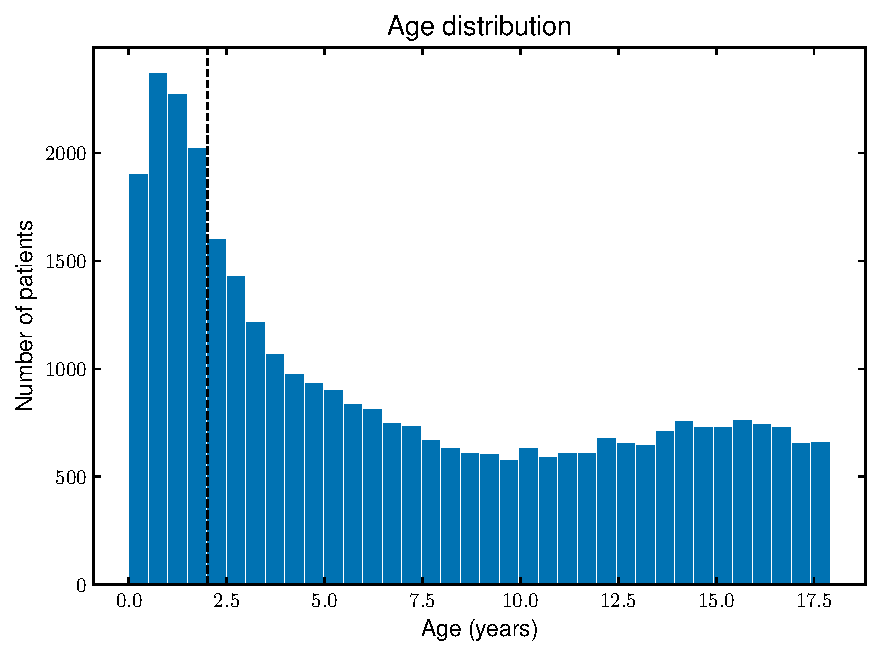
\includegraphics[width=0.65\textwidth]{../figs/eda_age_distribution.pdf}
    \caption{Age distribution of patients in the dataset}\label{fig: eda-age-distribution}
\end{figure}

We next examine the rate of ciTBI by GCS score. Recall that the dataset has already been filtered to only include patients with a total GCS score of 14 or 15.
We find that the ciTBI rate is substantially higher among patients with a GCS score of 14 (around 8\%) compared to patients with a GCS score of 15.
It is important to note, however, that the large majority of patients in the dataset have a GCS score of 15. This suggests that a GCS score of 14, or maybe other closely related factors such as altered mental status, 
could be quite indicative of elevated ciTBI risk. This conclusion would be consistent with the findings of \cite{Kuppermann2009};
their prediction rule explicitly incorporates altered mental status (defined as a GCS score of 14 or the presence of symptoms such as agitation, somnolence, repetitive questioning, or a slow response to verbal communication).



\begin{figure}[H]
    \centering
    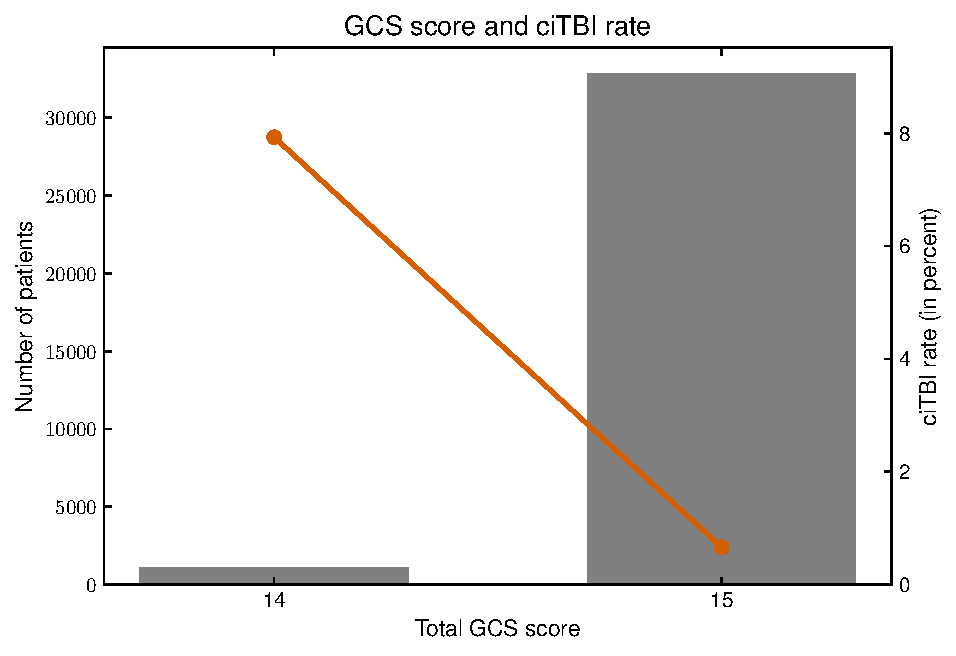
\includegraphics[width=0.65\textwidth]{../figs/eda_gcs_score.pdf}
    \caption{ciTBI rate by GCS score}\label{fig: eda-gcs-score}
\end{figure}



\begin{figure}[H]
    \centering
    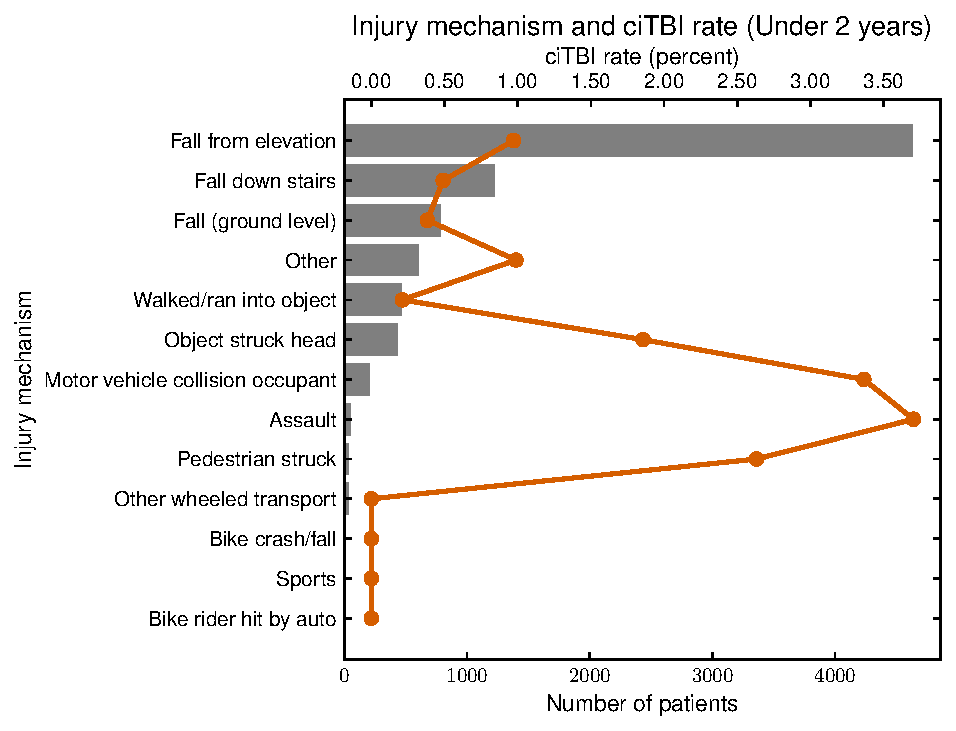
\includegraphics[width=0.65\textwidth]{../figs/eda_injury_mechanism_under2_years.pdf}
    \caption{Injury mechanisms and ciTBI rate for patients under 2 years old}\label{fig: eda-mechanism-citbi-under2}
\end{figure}

To get a sense of the various injury mechanisms present in the data and their associated severity, we plot the frequency of each injury mechanism along with the corresponding
ciTBI rate within each mechanism (Figure \ref{fig: eda-mechanism-citbi-under2} and \ref{fig: eda-mechanism-citbi-over2}). We stratify this visualization by age group,
as \cite{Kuppermann2009} suggests that the distribution and the risk profile of injury mechanisms can differ between younger and older children.
Indeed, we find that this is the case, although we note the limitation that some injury-mechanism categories contain very few patients, which can make the corresponding rate estimates unreliable.
That said, for patients under the age of 2, the ciTBI rate was especially high for motor vehicle collisions, assault, and pedestrians struck by a vehicle. For patients aged 2 and older,
the ciTBI rate was especially high for pedestrians struck by a vehicle, other wheeled-transport collisions, and bicycle riders struck by an automobile.

\begin{figure}[H]
    \centering
    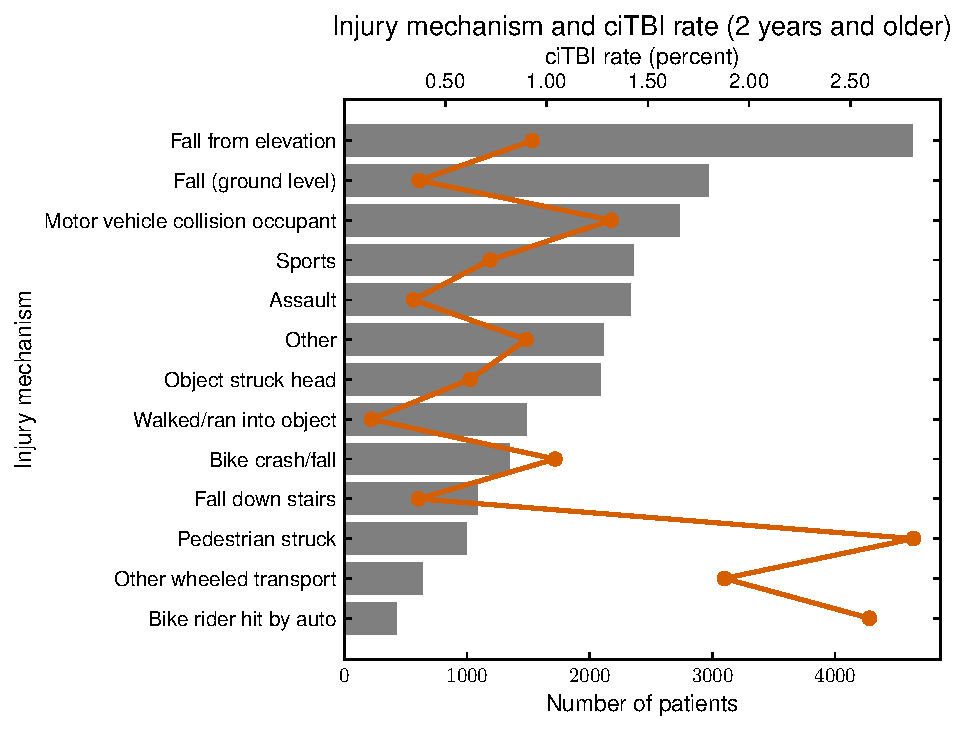
\includegraphics[width=0.65\textwidth]{../figs/eda_injury_mechanism_over2_years.pdf}
    \caption{Injury mechanisms and ciTBI rate for patients 2 years old and older}\label{fig: eda-mechanism-citbi-over2}
\end{figure}

One thing that stood out was that assault was a far more common injury mechanism (relative to each age group's data) among patients aged 2 and older than among patients under 2, yet
the ciTBI rate associated with assault was much higher in the younger group. This is consistent with domain knowledge: young children exposed to assault appear to be at substantially higher risk of ciTBI than older children exposed to the same mechanism.
As \cite{parker_traumatic_2021} note, ``a child is more vulnerable to a TBI than an adult due to unique physical attributes of the young brain and body. With a larger head to body ratio and weak musculature of the neck, the child's brain
is more likely to be exposed to greater acceleration/deceleration forces, resulting in a higher incidence of diffuse axonal injury and cerebral edema.''

For both age groups, falls from elevation and ground-level falls were common injury mechanisms overall, though they were not associated with particularly elevated ciTBI rates.
As a sanity check on the data, we can also see that there were no patients under the age of 2 with an injury mechanism of sports, bicycle crash/fall, or bicycle rider struck by automobile; hopefully, children under
the age of 2 are not riding bikes or playing sports, so this checks out with common sense.


Finally, to validate the motivating claims of the domain paper, we plot the overall proportion
of patients who received a CT scan alongside the overall ciTBI rate (Figure \ref{fig: eda-outcome-rates}). This is consistent with \cite{Kuppermann2009}: the CT usage rate (35.4\%) is far higher than the ciTBI rate (0.9\%).
This large gap between imaging rate and a measure of a true positive rate underscores the motivation for this analysis;
there appears to be room for improvement to develop a clinical decision rule in order to reduce unnecessary CT scans in this patient population.

Motivated by these summary visualizations, we further investigate the severity of the injury mechanism and symptoms like altered mental status (which is related
to GCS score of 14) on the empirical ciTBI rate in the dataset.

\begin{figure}[H]
    \centering
    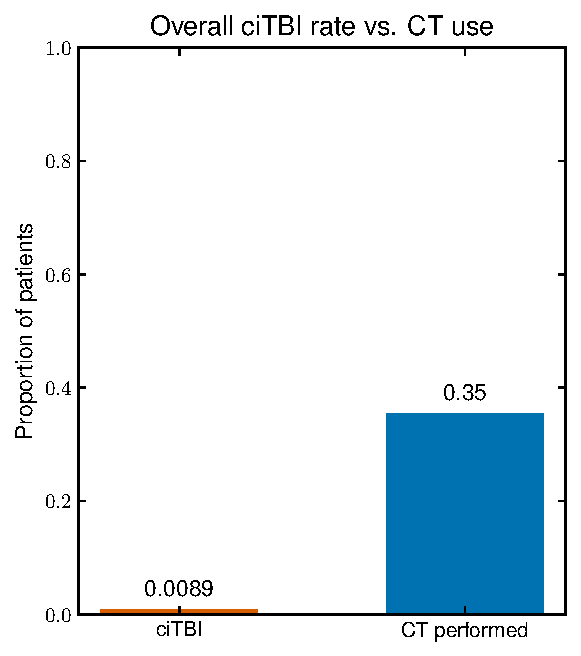
\includegraphics[width=0.50\textwidth]{../figs/eda_outcome_rates.pdf}
    \caption{Overall ciTBI rate vs. CT use}\label{fig: eda-outcome-rates}
\end{figure}

\section{Findings}\label{findings}

\subsection{First finding}\label{first-finding}

Our first finding is that the rate of CT scan usage is lower for black patients than
for white patients, across both age groups (Figure~\ref{fig: finding1-ct-race}). To produce this figure, we had to drop the 2,504 (7\%) observations missing the race variable.

One possible explanation is that non-black patients systematically present with more severe symptoms than black patients,
which would justify the discrepancy in imaging rates for clinical reasons. However, without evidence that this is the case,
this finding is consistent with the possibility of racial bias in the use of CT scans for pediatric head trauma patients.
If black and non-black patients in this dataset present with head trauma of comparable severity on average, then a gap
in imaging rates would suggest that physicians are applying a different threshold for ordering a CT scan depending on a patient's race (perhaps subconsciously).
This would be troubling for two reasons: under-imaging a genuinely high-risk patient risks a missed ciTBI diagnosis, while over-imaging a low-risk patient exposes that child to unnecessary ionizing radiation, which is precisely the harm that motivates
the development of the clinical decision rules in \cite{Kuppermann2009} in the first place.

However, we cannot conclude that racial bias is the cause of the observed discrepancy as this gap could be
explained by other differences in injury severity, mechanism, or timing in presentation to the emergency department.
Answering this question would require further investigation/analysis to determine which of the two possible explanations
is more consistent with the data. This is an important question to investigate as it provides insight into unnecessary use of
CT scans and where there can be potential reductions in CT scan usage.

Additionally, the sample sizes for the Pacific Islander and American Indian groups are comparatively much smaller, so it is difficult to draw any
conclusions about these two groups. We also note that, across all race groups, the proportion of patients receiving a CT scan was higher among patients aged
2 and older than among patients under 2. Again, this is consistent with domain knowledge: \cite{Kuppermann2009} implies
that CT scan use is less common in pediatric hospitals compared to non-pediatric hospitals, so it makes sense that children under the age of 2
have lower CT scan usage rates across the board.

\begin{figure}[]
    \centering
    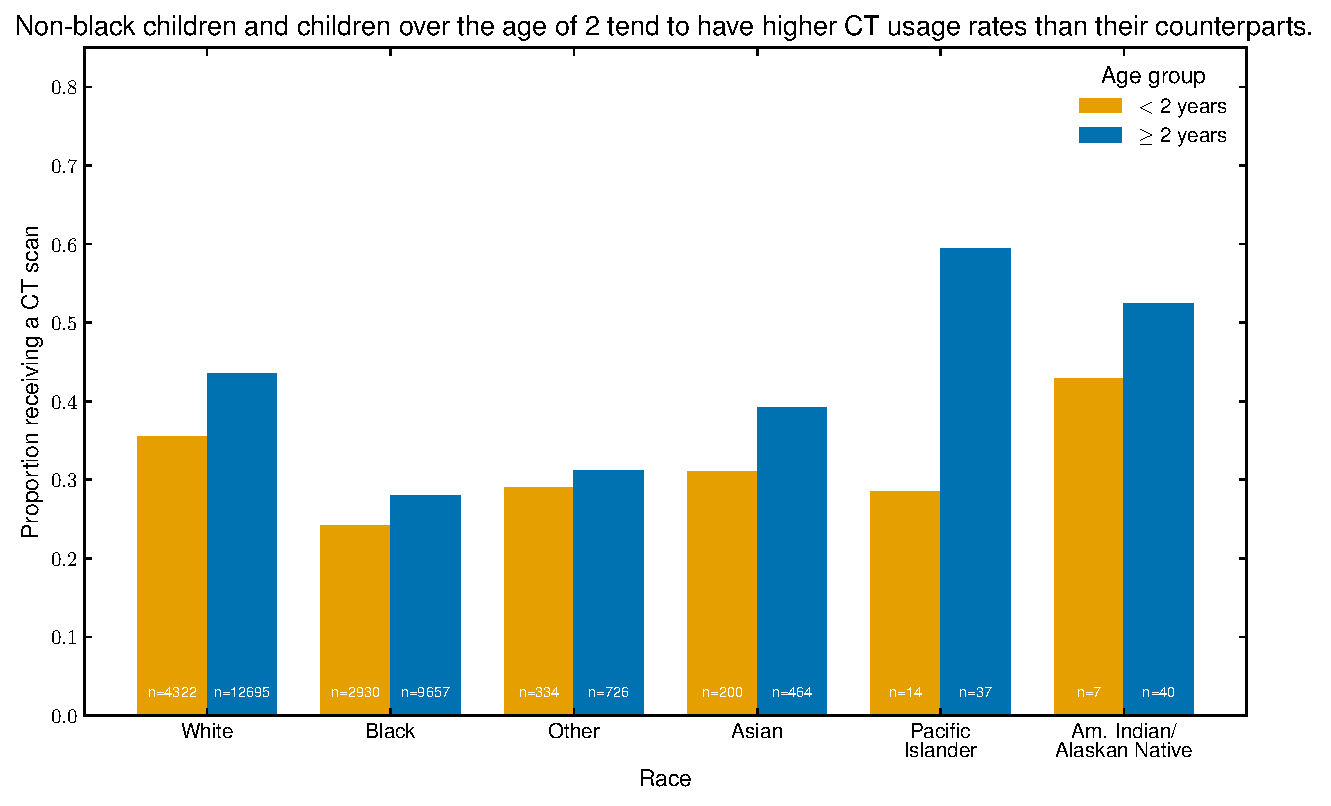
\includegraphics[width=0.75\textwidth]{../figs/ct_use_by_race_age.pdf}
    \caption{CT scan use by race and age. Non-black children and children $\geq$ 2 years old tend to have higher CT scan usage.}\label{fig: finding1-ct-race}
\end{figure}




\subsection{Second finding}\label{second-finding}

Our second finding is that clinical signs such as skull fracture and altered mental status are associated with a substantially higher rate of clinically-important TBI
than signs such as vomiting, headache, or scalp hematoma (Figure \ref{fig: finding2-risk-factors}). These signs appear highly predictive of ciTBI, and in fact
correspond exactly to the variables identified as ``branch points'' for high ciTBI risk in the clinical decision rules derived in \cite{Kuppermann2009}. These same signs also exhibit the
largest differential in ciTBI rate between the finding-absent and finding-present groups: for basilar skull fracture, the differential was 0.0079 versus 0.1387; for palpable skull fracture, it was 0.0073 versus 0.0739;
and for altered mental status, it was 0.0043 versus 0.0401.

For the purposes of this plot, we recoded ``suspected'' loss of consciousness as a present finding, and we excluded pre-verbal/non-verbal patients from the headache and amnesia variables,
since the ``not applicable'' code for these patients does not indicate a true absence of the symptom. We also plot the ciTBI rate on a log scale, since the rate spans
several orders of magnitude.

\begin{figure}[hbtp]
    \centering
    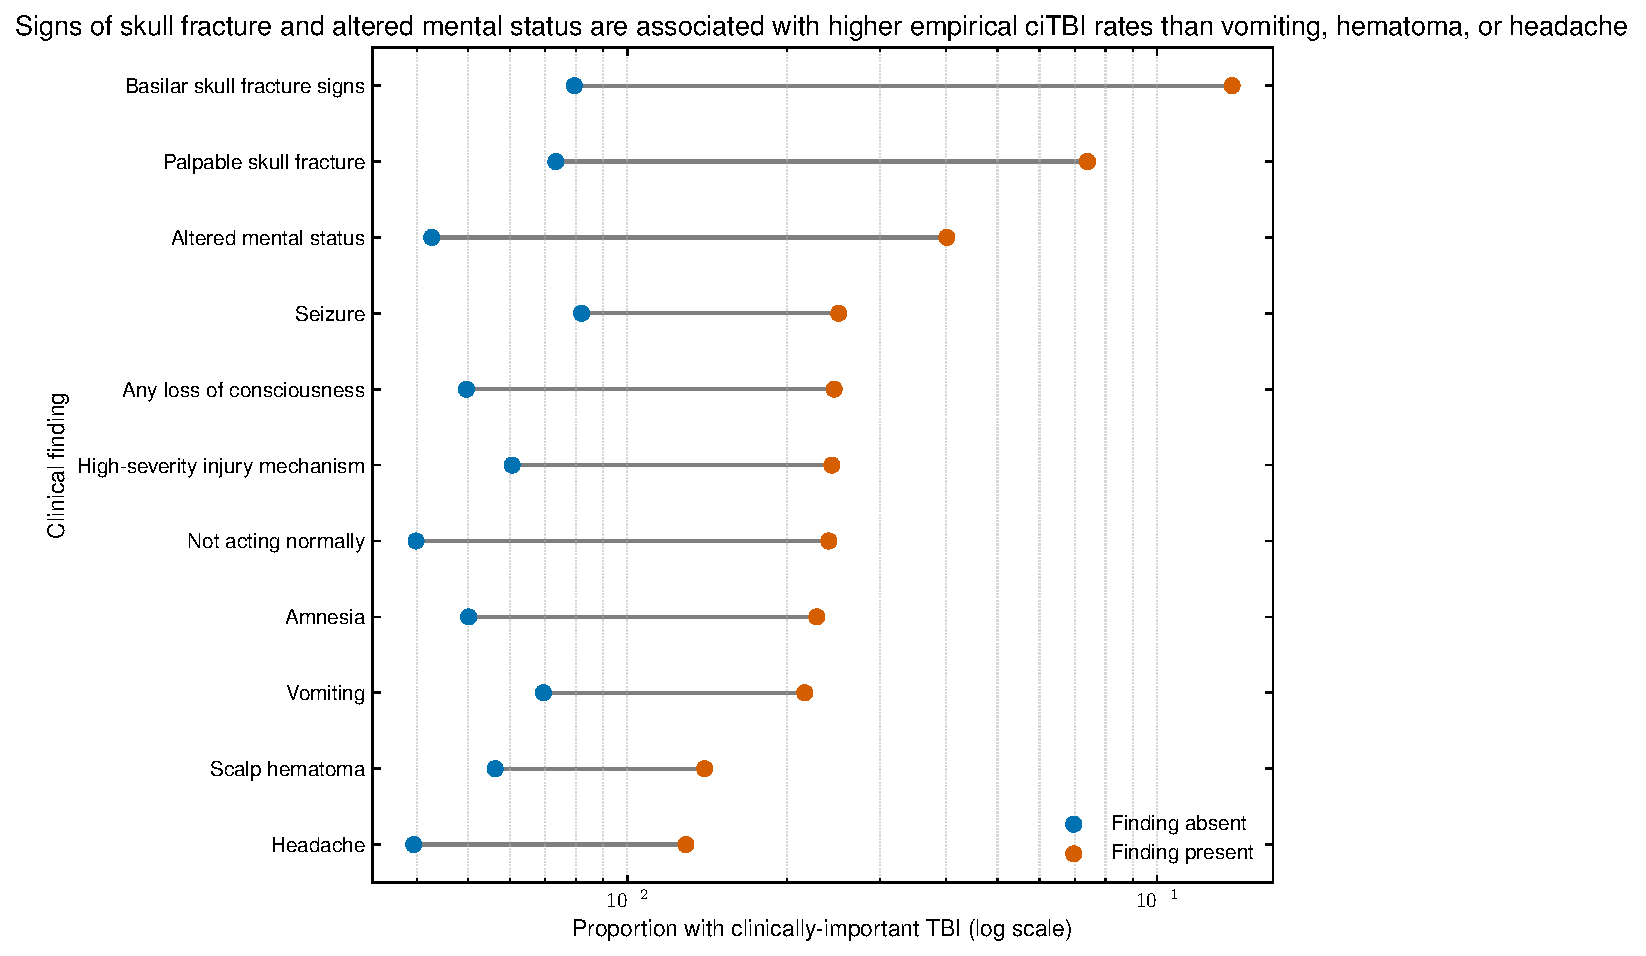
\includegraphics[width=0.90\textwidth]{../figs/clinical_risk_factors.pdf}
    \caption{ciTBI rate by presence of clinical findings. Clinical signs of skull fracture and altered mental status appear to be particularly associated with higher ciTBI rates.}\label{fig: finding2-risk-factors}
\end{figure}

\subsection{Reality Check}\label{reality-check}

Several aspects of the cleaned data line up with what we would expect from domain knowledge. For example, all of the patients in the dataset have an age in between 0 and 18 in the cleaned data (with the maximum being 17.92 years), which makes sense given that this is a dataset of pediatric patients.
Similarly, the GCS scores of our cleaned dataset all are either 14 or 15, and the subcomponents GCS eye, GCS verbal, and GCS motor all are within their expected
ranges (0-4, 0-4, 0-6) respectively. Second, the overall ciTBI rate in our cleaned data is low (0.9\%), which is consistent with \cite{Kuppermann2009} that only a small fraction of children presenting with minor head trauma go on to have a clinically significant brain injury.
Third, our overall CT usage rate (35.4\%) is quite a bit lower than the roughly 50\% national average cited in the literature; this is also consistent with domain knowledge, since \cite{Kuppermann2009} notes that the EDs participating in PECARN are predominantly pediatric hospitals, which typically have 
lower CT usage rates than general/non-pediatric hospitals. Fourth, the relationship between GCS score and ciTBI risk goes in the expected direction: patients with a GCS of 14 have a much higher ciTBI rate than patients with a GCS of 15, consistent with GCS 14 (and altered mental status more broadly)
being used as a branch point in the original decision rule in \cite{Kuppermann2009}. Finally, our injury-mechanism visualization also acts as a reality check: we do not observe any patients under 2 years old with an injury mechanism of sports, bicycle crash/fall, or being struck by a bicycle; this
is exactly as we would expect from common sense that children under 2 years old are not riding bikes or playing sports.
Thus, our cleaned data passes our reality check, and we do not see any issues that would suggest that the cleaned data is inconsistent with what we would expect from domain knowledge.


\subsection{Stability Check}\label{stability-check}

One judgment call that we made was when we were resolving the logical inconsistency for 884 observations that had a positive
palpable skull fracture indicator but a not-applicable value for the depression indicator. We treated these cases as missing values originally
for the depression indicator, but alternatively, we could have the left depression indicator as is and changed the value to NaN/missing
for the positive palpable skull fracture indicator. The original reasoning for this judgment call was that we thought that it was an encoding mistake to mark non-applicable for the depression
indicator if the patient was marked as positive for having a palpable skull fracture. We can check the stability of our findings by perturbing the data in this way and seeing how it affects our findings,
particularly in Figure \ref{fig: finding2-risk-factors}. Specifically, we can check if the ciTBI rate for palpable skull fracture is very different if which switch
which variable is marked as missing during the data cleaning for these odd observations (as the rates of ciTBI will be computed slightly differently for the finding present group). 

Refer to \ref{fig: finding2-risk-factors} for the original version. The perturbed version is shown in Figure \ref{fig: finding2-risk-factors-perturbed}.
We see that the position of the basilar skull fracture and palpable skull fracture have switched, with the ciTBI rate for the palpable skull fracture present
group being even higher than before. Previously, the ciTBI rate for the palpable skull fracture present group was 0.0739, but now it is 0.1641.
Thus, our finding that clinical signs of skull fracture and altered mental status are associated with higher ciTBI rates is stable to this perturbation, and in fact, the possible association is even stronger for palpable skull fracture
with this alternative judgment call.

\begin{figure}[hbtp]
    \centering
    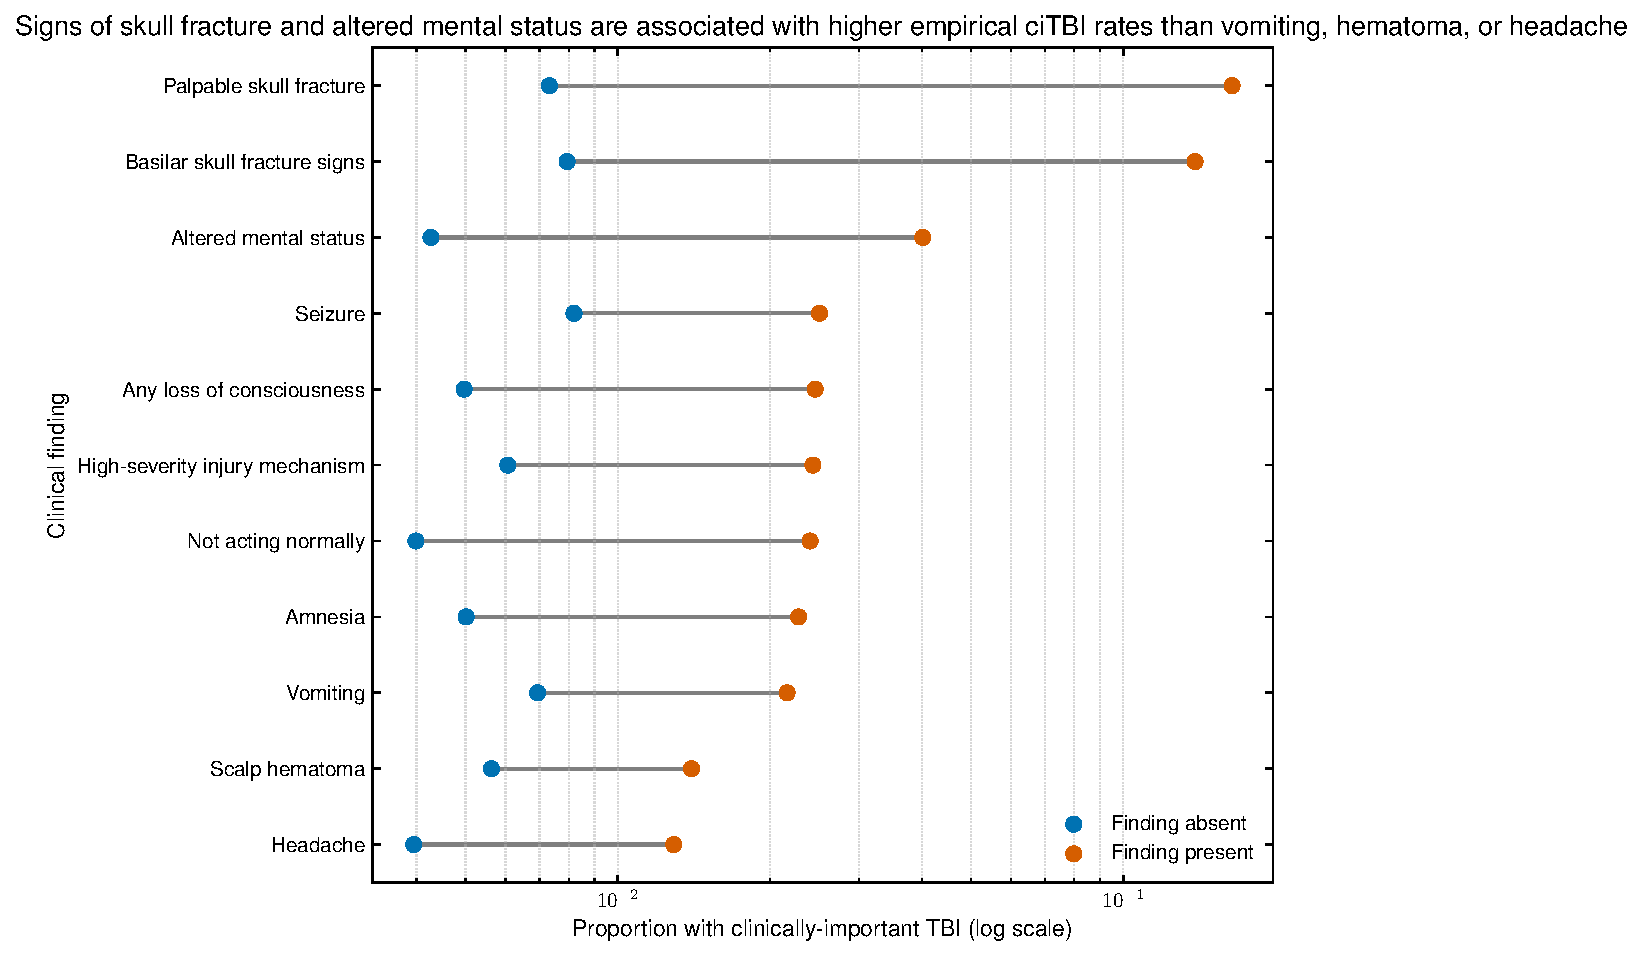
\includegraphics[width=0.90\textwidth]{../figs/clinical_risk_factors_perturbed.pdf}
    \caption{ciTBI rate by presence of clinical findings (perturbed data). Clinical signs of skull fracture and altered mental status appear to be particularly associated with higher ciTBI rates.}\label{fig: finding2-risk-factors-perturbed}
\end{figure}


\section{Modeling}

\subsection{Implementation}

We used two classification models to predict ciTBI: logistic regression and decision trees. These models were selected to provide
a comparison between a simple linear model vs. a more flexible non-linear model. Both models were trained using the training dataset
and then evaluated on a held-out validation dataset.

Before modeling, we dropped some variables that were not relevant to the prediction task, such as the patient numeric identifier, the individual ciTBI component variables,
and whether a CT scan was performed. Categorical variables were converted into binary indicator variables using one-hot encoding.
For logistic regression, missing numerical values were handled using median imputation.

Hyperparameters for both models were selected using grid search with five-fold stratified cross-validation
on the training dataset. We used stratified K-fold cross-validation to ensure that the proportion of ciTBI cases
was preserved across the folds. For logistic regression, the hyperparameters $C$ and class weight were optimized. The values considered for $C$ were $0.01$, $0.1$, $1$, and $10$,
and both the default class weighting and balanced class weighting were evaluated. For the decision tree, maximum depth, minimum samples per leaf, and class weight were optimized.
Maximum depth values of $2$, $3$, $4$, $5$, and unrestricted depth were considered, while minimum leaf sizes of $1$, $5$, $10$, and $20$ were evaluated.

The models were selected based on the criteria of harmonic mean of sensitivity and negative predictive value. This metric
was used because both sensitivity and NPV are important: a high sensitivity ensures that we are not missing patients with ciTBI, while a high NPV
enables us to be confident that patients predicted to not have ciTBI are actually low risk.

\subsection{Stability}

The stability of the models was evaluated using the data perturbation described in Section \ref{stability-check}.
The models were retrained on the perturbed training dataset and then evaluated on the held-out validation dataset (the full modeling process
was repeated with the perturbed data). Figure \ref{fig: model-stability} shows the sensitivity and NPV for each model on the original and perturbed datasets.
As can be seen, the model metrics did not change much under the perturbation, indicating that the models are stable to this perturbation.

\begin{figure}[hbtp]
    \centering
    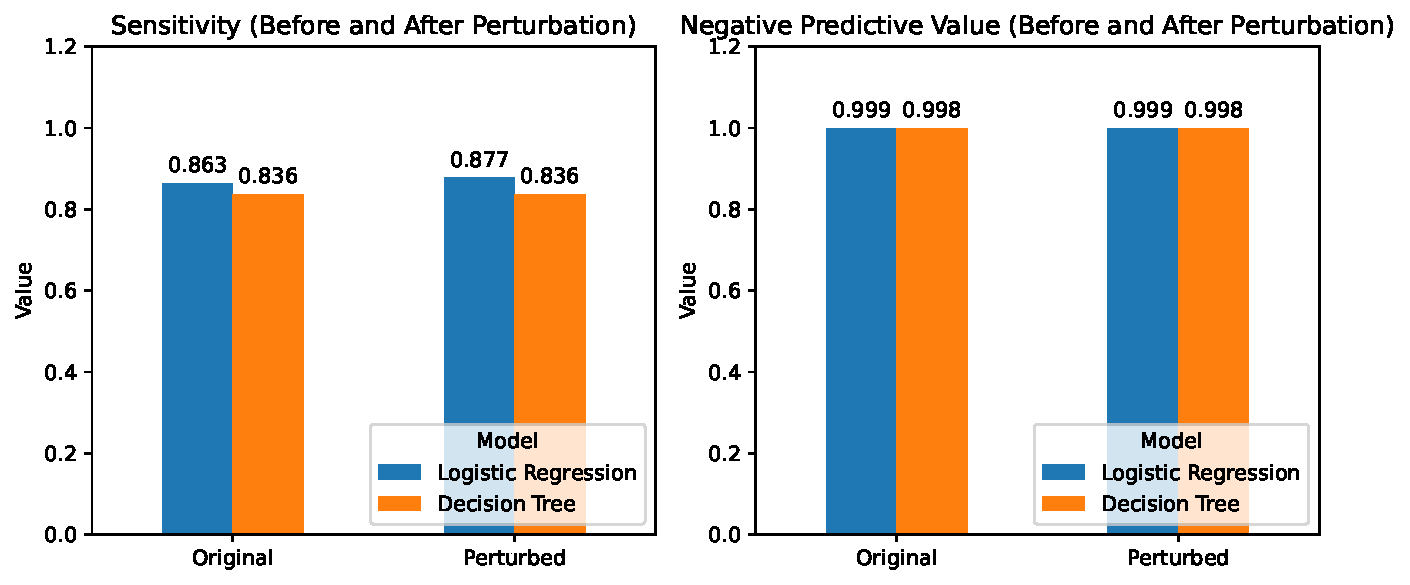
\includegraphics[width=0.75\textwidth]{../figs/model_stability.pdf}
    \caption{Sensitivity and NPV for each model on the original and perturbed datasets. The models are stable to the perturbation, as the metrics do not change much.}\label{fig: model-stability}
\end{figure}

\subsection{Discussion}

The two models were selected because they are both relatively interpretable and provide two different
approaches to the prediction problem. Logistic regression is a simple/linear baseline model, whereas
decision trees can capture non-linear relationships between the covariates and the outcome.

Both of these models can be interpreted in a straightforward manner. For logistic regression, we can simply look
at the associated coefficients for each covariate to understand its contribution to the model's estimated log-odds of ciTBI.
The decision tree can also be interpreted by tracing the path from the root node to the leaf node for a given observation,
which provides intuition for how the prediction is made. Both models can allow clinicians to see which features are used for predicting
risk of ciTBI. Figure \ref{fig: model-structure} shows the structure of the decision tree and how exactly the prediction is made.

\begin{figure}[]
    \centering
    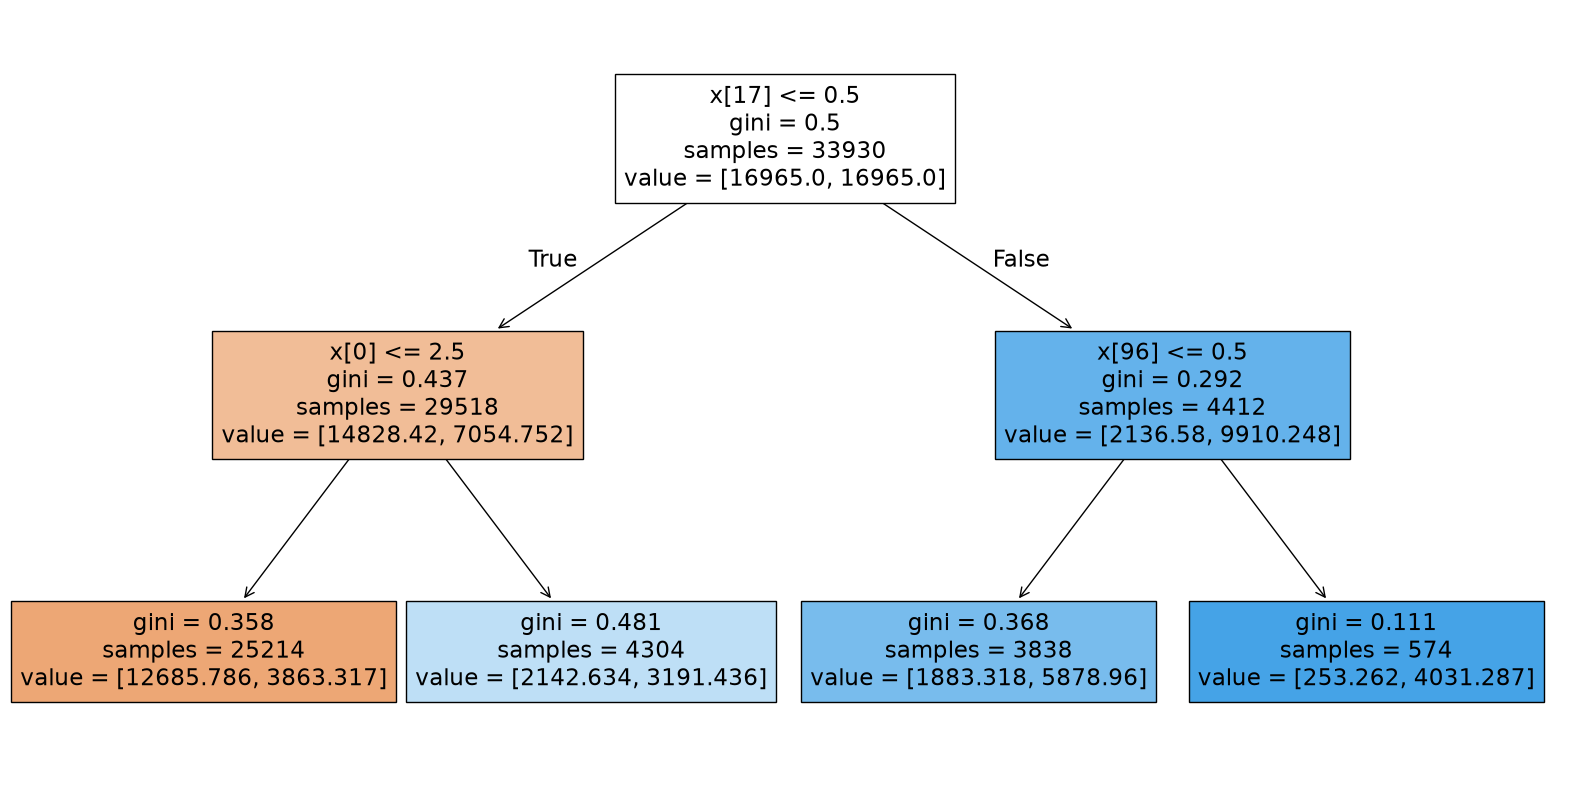
\includegraphics[width=0.75\textwidth]{../figs/decision_tree.png}\label{fig: model_structure}
    \caption{Decision tree structure. The decision tree can be interpreted by tracing the path from the root node to the leaf node for a given observation (assuming the labels are human-readable, in this case they are not).}\label{fig: model-structure}
\end{figure}

\section{Conclusion}\label{conclusion}

In this lab, we hoped to explore the PECARN TBI dataset to validate the clinical decision rule derived in \cite{Kuppermann2009} and to identify possible covariates that are predictive of ciTBI and/or CT scan usage.
We start in the real world with a domain problem: we want to reduce unnecessary CT scan usage and reduce children's exposure to radiation by identifying patients who are at low risk for ciTBI. In order to address this question, we use data collected from 25 emergency departments in PECARN.
To some degree, this data is inherently subjective, as it was collected by ED doctors who perceive and record patients differently. Additionally, the covariates that were collected represent only a small portion of the vast amount of information that could be relevant to predicting ciTBI or CT scan usage,
and most of that information was simply never collected. Still, the data is useful for our purposes, and it reflects reality to some degree. This is exactly where the second realm - the approximation of reality - comes in, and it is where our data falls. There is no one-to-one correspondence between data and reality:
there is simply too much information in the real world to capture in any dataset, and the data collection process is inherently susceptible to measurement error. Data visualization works with this same approximation of reality (the data), so there is likewise
no one-to-one correspondence between a data visualization and reality itself. But data visualization is still useful for showing us, and helping us learn, some truths about the world.
The analyses and statistical methods used in this project - the plots and EDA, as well as the decision trees and logistic regression used in our modeling - are all examples of algorithms and mental constructs, the third realm, that we as humans use to make sense of data and, through it, to make sense of reality. We can then apply these
methods and models to new data in hopes of convincing ourselves that our findings are generalizable and that we have learned something true about reality, which brings us back to the second realm, the approximation of reality.

Using the PCS principles of predictability and stability, we can assess whether our findings are robust to
perturbations of the data and are not simply spurious findings of one particular version of it; by checking that our findings align with domain knowledge and remain stable under reasonable alternative judgment calls, we can be somewhat more confident that we have learned something true about the world. In this case, we can
use these findings to inform clinical decision-making and make a real impact in the world, which brings us back to the first realm of reality. The modeling and EDA portion of the lab falls within the mental-construct/algorithm realm, whereas
the data cleaning is somewhere between approximating reality and the realm of algorithms.

The dataset was of a decent overall size, but there were relatively few ciTBI cases within it, which makes it harder to learn a model that generalizes well to new data and that learns something genuinely useful about predicting ciTBI, rather than overfitting to the small number of positive cases we do have.
Using the PECARN TBI dataset, we were able to validate the clinical decision rule derived in \cite{Kuppermann2009}, as many of the covariates used in that decision rule also appeared to be important and potentially associated with ciTBI risk in our own EDA. In addition, we found differences in CT scan usage by race and by age group,
which point to where there may be room for improvement in reducing unnecessary CT scans, which was the crux of the domain problem we wanted to solve.


\section{Academic honesty statement}\label{academic-honesty-statement}
To Professor Bin Yu: I affirm that all of the work and ideas displayed in this report are my own, and that I have performed all of the data analysis
procedures and written the code that underpins the analysis to the best of my ability and independently (with the exception of minor edits from LLMs to polish the code style, syntax, and documentation).
Any outside resources (including classmates, if applicable) that I have used to draft this report or perform the analysis described have been properly cited in the bibliography section.

I believe academic research honesty is foundational to the scientific method and scientific progress. If we, as researchers, are not honest, it poses a direct
threat to the pursuit of truth that we should be striving for as scientists. Furthermore, cherry-picking or falsifying results can cause a snowball effect of misinformation
that is detrimental to our understanding of the world and our ability to make data-driven decisions. It is also important to cite those whose ideas our work builds upon to give them
due credit for their contributions, just as I would like to receive credit for my own work. Thus, it is essential to practice academic honesty in the research world.


\section{Collaborators}\label{collaborators}
I did not have any classmate/informal collaborators on this assignment.

LLM Usage: I used GitHub Copilot to assist with writing docstrings/documentation and to improve the code style and syntax of my code. These were
mainly inline suggestions.


\bibliographystyle{plain}
\bibliography{references}

\end{document}
